
%(BEGIN_QUESTION)
% Copyright 2012, Tony R. Kuphaldt, released under the Creative Commons Attribution License (v 1.0)
% This means you may do almost anything with this work of mine, so long as you give me proper credit

Anta at motoren ikke starter når ``Run'' trykkes. En tekniker feilsøker med disse testene i rekkefølge:

$$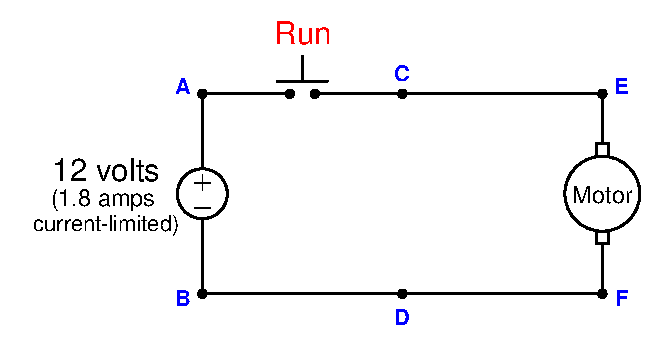
\includegraphics[width=15.5cm]{i00975x01.eps}$$

\begin{itemize}
\item{} {\bf Test 1:} 12 VDC mellom {\bf C} og {\bf D}, med ``Run'' trykket.
\vskip 25pt
\item{} {\bf Test 2:} 0 VDC mellom {\bf A} og {\bf C}, med ``Run'' ikke trykket.
\vskip 25pt
\item{} {\bf Test 3:} 12 VDC mellom {\bf A} og {\bf B}, med ``Run'' trykket.
\vskip 25pt
\item{} {\bf Test 4:} 12 VDC mellom {\bf E} og {\bf F}, med ``Run'' trykket.
\vskip 25pt
\item{} {\bf Test 5:} Uendelig ohm mellom {\bf E} og {\bf F}, med ``Run'' ikke trykket.
\vskip 25pt
\end{itemize}

Angi hvilken nyttig informasjon hver test gir (evt. ingen), og bestem feiltype/plassering så presist som mulig.

\underbar{file i00975}
%(END_QUESTION)





%(BEGIN_ANSWER)

{\bf Feilen er ``åpen krets'' mellom punkt E og F.}

%(END_ANSWER)





%(BEGIN_NOTES)

Testrekken peker på åpen feil i E-F-banen. Flere av målingene er overflødige etter at første/nøkkeltest allerede har avgrenset feiltypen.

%INDEX% Troubleshooting review: electric circuit diagnostic test rationale

%(END_NOTES)

